\documentclass[10pt,twocolumn,letterpaper]{article}

\usepackage[margin=0.75in]{geometry}
\usepackage{graphicx}
\usepackage{booktabs}
\usepackage{amsmath,amssymb}
\usepackage{textcomp}
\usepackage[hidelinks]{hyperref}
\usepackage{xcolor}
\usepackage{caption}
\captionsetup{font=small,labelfont=bf}
\newcommand{\dgr}{$^\circ$}

\title{\vspace{-1.5em}\textbf{Conv-ChArT: A Convolutional--Transformer Hybrid for\\
Accurate and Compact Fiducial Corner Detection and Pose Estimation}\vspace{-0.5em}}
\author{}
\date{}

\begin{document}

% Title and abstract occupy their own single-column page; the body begins two-column overleaf.
\onecolumn
\maketitle
\thispagestyle{empty}
\vspace{2em}
\begin{abstract}
\noindent
Fiducial-marker pose estimation underpins a wide range of localisation tasks, from camera
calibration and motion capture to visual servoing, augmented reality and mobile-platform
navigation. Existing detectors fail in complementary ways: classical corner-based pipelines are
accurate but abstain on a large fraction of degraded frames, while learned detectors sustain
throughput by emitting confidently wrong poses. We present Conv-ChArT, a convolutional--transformer
hybrid for ChArUco corner detection and pose estimation. A convolutional encoder--decoder is
coupled to a multi-head self-attention bottleneck with axial rotary position encoding, supplying
board-scale context that a convolutional receptive field alone cannot reach across a scale envelope
spanning more than a decade in apparent board size; identity is predicted by a dedicated class map,
corners are localised sub-pixel by a compact confidence-gated refinement network, and a
lattice-consistency homography gate makes abstention an explicit, geometrically justified outcome.
We evaluate against two baselines: the standard classical ChArUco pipeline, and the established
learned baseline for this task, a two-stage convolutional system that predicts corners and
identities on a coarse grid, which we fine-tune on our data; as in that system's own coarse
evaluation, its second-stage refinement network is not run.
Conv-ChArT establishes a new accuracy--efficiency operating point against both. Our full pipeline
uses \textbf{2.3$\times$ fewer parameters} than the learned baseline, yet reduces median pose
rotation error by \textbf{6.9$\times$} and 95th-percentile rotation error by \textbf{76$\times$}; a
variant using \textbf{7.0$\times$ fewer parameters} still surpasses it on every accuracy metric.
The disparity between median and tail improvement reflects the two systems' failure modes: the
baseline sustains throughput by fitting poses to inconsistent correspondences, whereas our
geometric gate declines them. On corner localisation our reference model attains 0.4063\,px median
and 0.6733\,px 95th-percentile error at 99.53\% identification accuracy. We release three width
tiers, characterise them over twenty degradation factors, and report all ablations against a
measured per-width reproducibility floor.
\end{abstract}
\clearpage
\twocolumn

%---------------------------------------------------------------
\section{Introduction}

Planar fiducial markers remain the standard instrument for establishing metric camera pose from a
single view, and underpin a wide range of localisation tasks: extrinsic and intrinsic camera
calibration, multi-camera and camera-to-sensor registration, object and platform tracking, visual
servoing, motion capture, and augmented-reality anchoring. The ChArUco board, a chessboard whose
white squares carry ArUco markers, combines the sub-pixel localisability of chessboard saddle
points with the identifiability of coded markers, and is the default choice where accuracy matters.
The classical detection pipeline is a sequence of hand-designed stages: adaptive threshold,
quadrilateral extraction, marker decoding and corner interpolation. Each stage is individually
interpretable and collectively brittle, since a failure at any point removes the corner entirely.

Learned detectors address this brittleness by regressing corner locations directly from pixels.
Deep ChArUco~\cite{hu2019} demonstrated that a convolutional network recovers ChArUco corners in
illumination regimes where the classical pipeline abstains entirely. The learned formulation,
however, introduces a failure mode the classical one does not have. A classical pipeline that
cannot decode a marker reports nothing; a learned detector always emits a heatmap, and a downstream
solver will fit \emph{some} pose to whatever peaks it contains. Wherever the pose is consumed
automatically, whether by a calibration that is never inspected, a tracking filter or a control
loop, a confidently wrong pose is categorically worse than no pose, because nothing downstream can
distinguish it from a correct one.

Conv-ChArT is designed so that accuracy and abstention are obtained together, at a parameter budget
compatible with embedded deployment. We make the following contributions.

\begin{itemize}\itemsep2pt \parskip0pt \topsep2pt
\item \textbf{We present} a convolutional--transformer detector in which a self-attention
bottleneck with axial rotary position encoding supplies board-scale context, and identity is
predicted by a dedicated class map. Its full pipeline uses 979,458 parameters against 2,245,992
for the learned baseline, and is more accurate on every metric we measure (Sec.~\ref{sec:pose});
the bottleneck itself is ablated in Sec.~\ref{sec:ablation} (\emph{Attention bottleneck}).
\item \textbf{We show} that supervising the corner heatmap with a one-hot target under binary
cross-entropy outperforms the Gaussian-target penalty-reduced focal loss conventional in dense
keypoint detection, and that the two heads are best supervised differently
(Sec.~\ref{sec:ablation}, \emph{Supervision signal}).
\item \textbf{We introduce} two geometric gates: a refinement stage applied only where its own
predicted confidence supports it, and a lattice-consistency homography test that converts
inconsistent correspondences into an explicit refusal rather than a pose
(Sec.~\ref{sec:ablation}, \emph{Geometric gating}).
\item \textbf{We propose} reporting ablations against a measured per-width reproducibility floor
obtained from repeated identical training runs. The smallest resolvable effect depends jointly on
width and metric, varying across the widths we train by $11.6\times$ in 95th-percentile
localisation and $88\times$ in identity (Sec.~\ref{sec:ablation},
\emph{Reproducibility floor}).
\end{itemize}

%---------------------------------------------------------------
\section{Related Work}

\textbf{Fiducial markers and classical detection.}
Square-marker systems~\cite{artoolkit,artag,apriltag,aruco} encode identity in a binary grid and
recover pose from four corners. ChArUco boards interleave markers with a chessboard so that saddle
points, which localise far more precisely than marker corners, inherit identity from neighbouring
markers. The OpenCV implementation is the de facto reference and forms one of our baselines.

\textbf{Learned keypoint detection.}
Our heatmap formulation follows the dense-prediction lineage of CornerNet~\cite{cornernet} and
CenterNet~\cite{centernet}, in which keypoints are supervised as Gaussian-smoothed targets and
decoded by local-maximum extraction. We adopt the loss-normalisation convention of that lineage but
depart from its target representation, for reasons established in Sec.~\ref{sec:abl_sup}.

\textbf{Learned fiducial detection.}
Deep ChArUco~\cite{hu2019} is the closest prior work: a two-headed convolutional network predicting
corner locations and identities on a coarse cell grid, with a separate refinement network. We adopt
its two-stage decomposition and use it as our learned baseline. Conv-ChArT differs in the attention
bottleneck, the full-resolution heatmap head, the geometric gate, and a substantially smaller
parameter budget.

\textbf{Attention in dense prediction and gating.}
Self-attention bottlenecks in U-Net-style encoders~\cite{unet} are established in segmentation. We
use a pre-norm transformer block with axial rotary position embedding~\cite{roformer,ropevit},
chosen so that the encoding is relative and the exported graph remains free of operators
unsupported by embedded inference runtimes. We adopt the additive attention gate of Attention
U-Net~\cite{attnunet} on the finest skip connection, with its pass-through initialisation.

%---------------------------------------------------------------
\section{Method}

We first define the task and notation (Sec.~\ref{sec:formulation}), then describe the network
(Sec.~\ref{sec:arch}, overviewed in Fig.~\ref{fig:arch}), its supervision (Sec.~\ref{sec:sup}), the
refinement and geometric stages that produce a pose or a refusal (Sec.~\ref{sec:geom}), and the
training configuration (Sec.~\ref{sec:impl}).

\begin{figure*}[t]
\centering
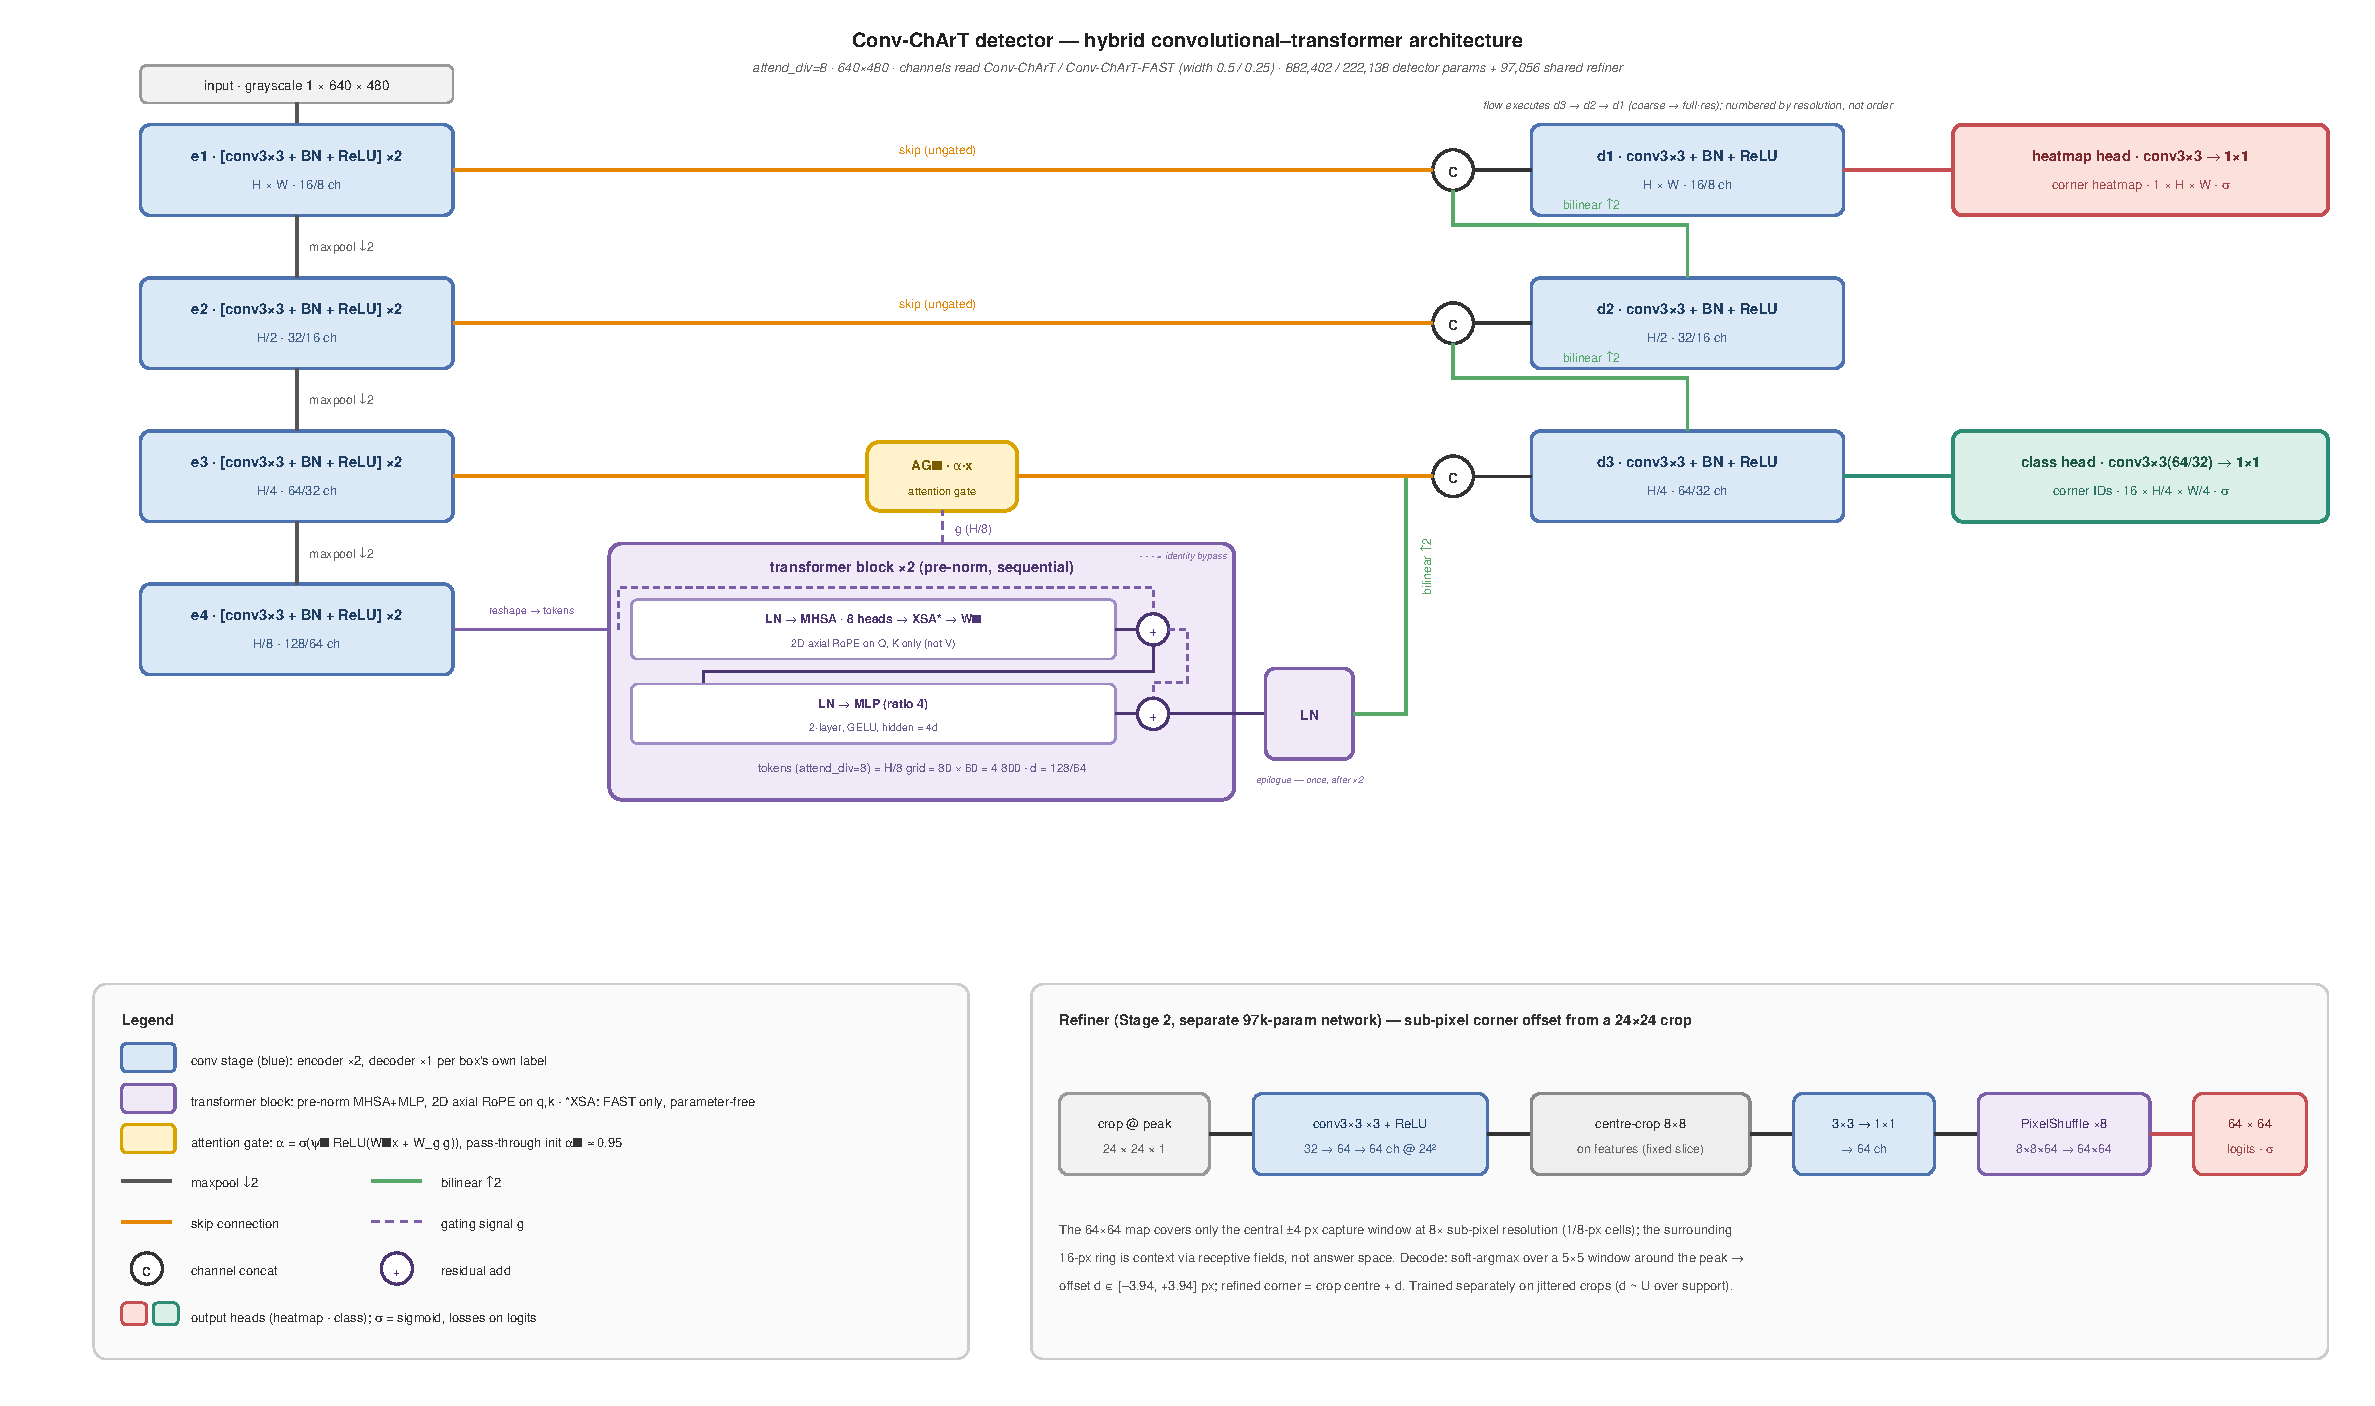
\includegraphics[width=0.92\textwidth]{figs/architecture.pdf}
\caption{\textbf{Conv-ChArT architecture.} A grayscale frame enters a four-stage convolutional
encoder; the deepest feature map is reshaped into an $80\times60$ token grid and passed through two
pre-norm self-attention blocks with axial rotary position encoding, which supply the board-scale
context that sets identity. A three-stage bilinear decoder recombines the attended features with
encoder skips, the finest of which passes through an additive attention gate. Two heads emit a
full-resolution corner heatmap and a 16-channel identity map at $H/4$. Peaks from the heatmap are
cropped and refined sub-pixel by a separate 97,056-parameter network; identities are read from the
class map at the coarse peak locations, tested for mutual consistency against a board homography,
and either solved for pose or refused. The attention bottleneck holds 44.9\% of the 882,402
parameters.}
\label{fig:arch}
\end{figure*}

\subsection{Problem definition and notation}
\label{sec:formulation}

Given a grayscale frame $I \in \mathbb{R}^{H \times W}$ containing a $5\times5$ ChArUco board with
$n = 16$ interior corners, we recover the image positions $\mathbf{x}_i \in \mathbb{R}^2$ and board
indices $c_i \in \{1,\dots,n\} \cup \{\varnothing\}$ of the visible corners, and the camera pose
$(\mathbf{R},\mathbf{t}) \in SE(3)$. The system may decline to report a pose. Formally,

\begin{equation}
f(I) \;=\; \big(\{(\mathbf{x}_i, c_i)\}_{i=1}^{K},\; (\mathbf{R},\mathbf{t}) \cup \{\varnothing\}\big),
\label{eq:signature}
\end{equation}

with $K$ the number of detected corners, $c_i = \varnothing$ for a detection whose identity is not
established, and the pose term $\varnothing$ when the correspondences fail the consistency test of
Sec.~\ref{sec:geom}. We write $s$ for the apparent board square size in pixels; the operating
envelope is $s \in [12,128]$.

\textbf{Refusal is an output, not a failure.} A learned detector always produces a heatmap, so a
pose solver downstream will always return something. Eq.~\ref{eq:signature} makes the refusal
explicit and typed, which is what allows the error distribution to be bounded rather than merely
centred (Sec.~\ref{sec:pose}).

\textbf{Half-pixel convention.} Every resolution change uses $x' = (x + 0.5)r - 0.5$. Class-map
readout uses bilinear sampling with \texttt{align\_corners=False}, algebraically identical to
mapping into cell space by $(x+0.5)/4 - 0.5$; dividing coordinates by 4 instead is biased by 0.375
cells, or 1.5\,px at input resolution. Coordinates are float64 throughout, with no integer cast
between the analytic corner and the training target.

\subsection{Architecture}
\label{sec:arch}

\textbf{Encoder.} Four stages, each a pair of $3\times3$ Conv--BN--ReLU with stride-2 downsampling
between stages, at width multiplier 0.5. The deepest stage is a plain convolutional stage. An
earlier variant used a dilated cascade there to extend the receptive field; it is redundant once
attention supplies board-scale context, and removing it costs nothing measurable while saving 25\%
of parameters (Sec.~\ref{sec:abl_attn}).

\textbf{Attention bottleneck.} The $H/8$ feature map is reshaped, without patch embedding, class
token or absolute position embedding, into an $80\times60$ grid of 4800 tokens and passed through
two pre-norm transformer blocks with 8 heads. Position is encoded by axial rotary
embedding~\cite{roformer,ropevit} with wavelengths geometric over $[2.5,\,2\max(H',W')]$ cells. The
longest wavelength exceeding twice the grid extent makes the joint phase code injective over all
in-frame offsets, so a distant token pair cannot alias onto a near one. This bottleneck is the sole
board-scale context mechanism, and is what makes identity recoverable at large $s$, where a
corner's own neighbourhood contains no marker.

\textbf{Decoder and heads.} Three bilinear-upsampling stages with skip concatenation. The finest
skip passes through an additive attention gate~\cite{attnunet} initialised to pass-through, gating
only where the recovery pass of Sec.~\ref{sec:geom} can undo an incorrect veto. A full-resolution
heatmap head and a 16-channel class map at $H/4$ terminate the network; final logit convolutions
are bias-initialised to $-2.19$ following~\cite{cornernet,centernet}. We note this is not
prior-matched to our task: $\sigma(-2.19) = 0.1006$ against a one-hot positive rate of
$16/307{,}200 \approx 5.2\times10^{-5}$, so the initialisation is inherited rather than derived,
and a matched value would be near $-9.9$. We did not ablate it.

Table~\ref{tab:params} gives the parameter distribution. We release two further tiers at width
multipliers 0.375 and 0.25. The 502k tier is identical in topology to the reference; the 222k tier
additionally enables exclusive self-attention (XSA) in the bottleneck, a parameter-free variant in
which a token is excluded from its own attention distribution. At that width XSA measures
$-0.0040$\,px p95 and $+0.21$\,pp identity against an otherwise identical control, both well
inside that width's reproducibility floor (Table~\ref{tab:floor}); we adopt it because it is free,
not because the difference is resolvable, and state it as such. This is why the 222k export carries
284 ONNX nodes against 263 for the other two tiers (Sec.~\ref{sec:deploy}).

\begin{table}[t]
\centering\small
\begin{tabular}{lrr}
\toprule
Module & Parameters & Share \\
\midrule
Transformer blocks & 396,544 & 44.9\% \\
Encoder stage 4 & 221,696 & 25.1\% \\
Decoder stage 3 & 110,720 & 12.5\% \\
Encoder stage 3 & 55,552 & 6.3\% \\
Class head & 37,968 & 4.3\% \\
Decoder stage 2 & 27,712 & 3.1\% \\
Encoder stage 2 & 13,952 & 1.6\% \\
Decoder stage 1 & 6,944 & 0.8\% \\
Attention gate & 6,209 & 0.7\% \\
Encoder stage 1 & 2,512 & 0.3\% \\
Heatmap head & 2,337 & 0.3\% \\
\midrule
Detector total & 882,402 & \\
Refiner (separate network) & 97,056 & \\
\bottomrule
\end{tabular}
\caption{Parameter distribution of the reference model.}
\label{tab:params}
\end{table}

\subsection{Supervision}
\label{sec:sup}

Let $\hat p$ denote a predicted probability and $Y$ the target at the same location. The heatmap
head is supervised by binary cross-entropy against a one-hot target, in which only the pixel
nearest each visible corner is positive:

\begin{equation}
\mathcal{L}_{\mathrm{hm}} = -\!\!\sum_{\mathbf{x}}\Big[\,\mathbb{1}[Y{=}1]\log\hat p
\;+\; \mathbb{1}[Y{<}1]\log(1-\hat p)\,\Big].
\label{eq:bce}
\end{equation}

The class head is supervised by the penalty-reduced focal loss of~\cite{cornernet} against a
Gaussian target of width $\sigma_{\mathrm{cls}}$:

\begin{equation}
\mathcal{L}_{\mathrm{cls}} = -\!\!\sum_{\mathbf{x}}
\begin{cases}
(1-\hat{p})^{\alpha}\log \hat{p}, & Y = 1,\\[2pt]
(1-Y)^{\beta}\,\hat{p}^{\alpha}\log (1-\hat{p}), & Y < 1,
\end{cases}
\label{eq:focal}
\end{equation}

with $\alpha = 2$, $\beta = 4$. Both are computed in logit space. The naive form is unusable in
bf16 not through underflow, since bf16 carries fp32's 8-bit exponent, but through mantissa
precision: with 8 mantissa bits, $1 - \hat p$ rounds to zero once $\hat p \gtrsim 1 - 2^{-9}$,
which the forced target peaks drive it to. The total objective is

\begin{equation}
\mathcal{L} = \frac{1}{N}\Big[\, \mathcal{L}_{\mathrm{hm}}
+ \lambda_{\mathrm{cls}}\,\mathcal{L}_{\mathrm{cls}} \,\Big],
\qquad N = \max\!\Big(\textstyle\sum_b N_b,\, 1\Big),
\label{eq:total}
\end{equation}

where $N$ is the batch-total count of visible corners, shared by both heads and clamped at one so
that all-negative batches require no special case.

Eq.~\ref{eq:focal} reduces to Eq.~\ref{eq:bce} when $\alpha=0$ and $Y\in\{0,1\}$. Using the
one-hot form on the heatmap departs from the convention of~\cite{cornernet,centernet}; it improves
localisation because the graded target's proximity discount makes displaced probability mass nearly
free, which we isolate in Sec.~\ref{sec:abl_sup}. The two smaller tiers use Eq.~\ref{eq:bce} for
both heads; $\lambda_{\mathrm{cls}}$ is 2.0 at the reference and 222k widths and 1.5 at 502k.

\subsection{Refinement, correspondence and pose}
\label{sec:geom}

\textbf{Sub-pixel refinement.} Peaks are decoded from the heatmap by $3\times3$ max-pool equality,
deduplicated within 2\,px, and capped at 64. A separate 97,056-parameter network takes a
$24\times24$ crop centred on each peak and predicts a $64\times64$ logit map, decoded by a
probability-weighted centroid over a $5\times5$ window around the argmax. The refiner never
upsamples its input; resolution is gained by pixel-shuffling learned channels, which keeps the
exported graph free of resize operators.

\textbf{Confidence gate.} Refinement is applied only where the refiner's own peak confidence
exceeds 0.3; below that the coarse peak is retained. The refiner is worse than the coarse peak on
16.3\% of crops, predominantly those without recoverable corner structure, and no amount of
training recovers a sub-pixel position from a crop that does not contain the corner. We gate on
the refiner's own output rather than on an image statistic so the decision uses the same evidence
the refinement does; the gate is ablated in Sec.~\ref{sec:ablation} (\emph{Geometric gating}).

\textbf{Identity readout.} Identity is read from the class map at the \emph{coarse} peak positions.
The class map is at $H/4$, so sub-pixel position carries no identity information; more importantly,
the gate and recovery pass below both reassign identity on the strength of positions, so feeding
them refined coordinates would let the refiner rewrite identity indirectly. Decoupling makes the
refined and unrefined arms bit-identical in identity by construction.

\textbf{Lattice-consistency gate.} A homography is fitted by RANSAC from the identified corners to
the canonical board lattice. Corners inconsistent with the fit are demoted; a recovery pass then
re-projects all board corners through the homography to assign identities the class head missed.
Degenerate configurations, namely fewer than four identified corners, collinear sets, and
exact-four fits that are vacuous by construction, yield typed refusals rather than a pose. Pose is
solved by IPPE~\cite{ippe} on undistorted coordinates, with an ambiguity flag raised when the two
IPPE solutions' reprojection errors are within a factor of 1.5. The flag fires on 4.2/4.1/4.6\% of
solved frames across our three tiers and is reported rather than acted on: it is a second,
softer refusal channel that a consumer may use to discount a pose without discarding it.

\subsection{Implementation details}
\label{sec:impl}

Table~\ref{tab:hyper} gives the training configuration; all three tiers share it. Training runs in
PyTorch 2.8 on a single RTX 5090 and takes 8.4\,h for the 882k and 502k tiers and 9.4\,h for the
222k tier; the refiner is trained separately (1.7\,h). Training data is generated on the fly.
Appendix~\ref{app:impl} gives the loader configuration, the full architecture specification, and
the determinism and provenance machinery.

\begin{table}[t]
\centering\small
\begin{tabular}{ll}
\toprule
Input resolution & $640\times480$, grayscale \\
Steps & 100,000 (detector), 10,000 (refiner) \\
Batch & 16 $\times$ 2 accumulation (effective 32) \\
 & 512 (refiner) \\
Optimiser & AdamW, $\beta = (0.9, 0.999)$ \\
Peak / floor LR & $3\times10^{-4}$ / $3\times10^{-6}$ \\
Schedule & cosine, 1000 warmup steps \\
Weight decay & $10^{-4}$, excl.\ biases and norms \\
Gradient clip & 5.0 \\
EMA decay & 0.999 (evaluated) \\
Precision & bf16 autocast, fp32 master weights \\
\bottomrule
\end{tabular}
\caption{Training configuration, shared by all three tiers.}
\label{tab:hyper}
\end{table}

%---------------------------------------------------------------
\section{Experiments}

\subsection{Data, metrics and baselines}
\label{sec:setup}

\textbf{Training data.} No annotated corpus exists at the scale and degradation severity needed to
characterise behaviour across the operating envelope, and manual sub-pixel annotation of chessboard
saddle points is infeasible at the precision the task demands. We train entirely on synthetic
composites with analytically exact labels: a rendered board is warped by a sampled homography onto
a natural-image background, alpha-composited, occluded, and photometrically degraded, with corner
positions computed through the same homography rather than from pixels. Apparent square size is
log-uniform over $[12,128]$\,px and perspective is sampled as a physical tilt up to 60\dgr.
Appendix~\ref{app:data} details the photometric model and labelling policy.

\textbf{Metrics.} \textbf{M-01} is the localisation error of matched corners under greedy
nearest-neighbour matching within 8\,px, reported as median and 95th percentile.
\textbf{Tail\,$>$\,4\,px} is the fraction of matched corners outside the refiner's capture radius,
our operational gate. \textbf{M-02} is match ratio by scale octave. \textbf{M-04} is corner
identification accuracy, conditioned on detection; a model detecting fewer, easier corners is
scored on an easier set, so we report recall alongside it throughout. \textbf{M-05/M-06} are pose
rotation (geodesic) and translation error, the latter in board squares.

\textbf{Baseline provenance.} The classical baseline is the OpenCV ChArUco pipeline at default
detector parameters. The learned baseline is Deep ChArUco~\cite{hu2019}; we did not copy its
published numbers, which were obtained on a different distribution. We initialised from the public
reference checkpoint, reinitialised the identity head for our board dictionary, and fine-tuned on
our training distribution under the same early-stopping criterion applied to our own arms,
terminating at 62,458 steps on convergence. Its corners pass through the identical
correspondence-gating and pose stage as ours, so the comparison isolates corner quality rather than
pose-solver implementation. Its refinement network is not run, which we state rather than hide; its
$320\times240$ input against our $640\times480$ is a further asymmetry.

\subsection{Corner detection}
\label{sec:detect}

\begin{table}[t]
\centering\small
\setlength{\tabcolsep}{4pt}
\begin{tabular}{lrrrrrr}
\toprule
Tier & Params & p95 & Median & M-04 & Tail & Far-oct. \\
 & & (px) & (px) & (\%) & (\%) & rec.\ (\%) \\
\midrule
222k & 222,138 & 0.734 & 0.413 & 99.09 & 0.019 & 87.5 \\
502k & 502,322 & 0.689 & 0.408 & 99.41 & 0.015 & 90.5 \\
\textbf{882k} & 882,402 & \textbf{0.673} & \textbf{0.406} & \textbf{99.53} & \textbf{0.005} & \textbf{91.7} \\
\midrule
\emph{floor, 222k} & & 0.023 & & 6.18 & 0.010 & \\
\emph{floor, 882k} & & 0.002 & & 0.07 & 0.005 & \\
\bottomrule
\end{tabular}
\caption{Corner detection, full 10,000-sample validation at 100,000 steps, with the seed-to-seed
floor of Table~\ref{tab:floor} repeated at the ladder's two endpoints. Figures are quoted to one
digit past the 882k floor. Far-octave recall is M-02 in the $s = 64$--128 bin.}
\label{tab:detector}
\end{table}

Table~\ref{tab:detector} reports the three released tiers. Across a $4\times$ parameter range,
in-envelope identity spans 0.44\,pp and median localisation 0.0065\,px; both are inside the 222k
floor and so are not resolvable at the ladder's lower end. Of the three separations that do exceed
it, the 95th percentile ($+0.060$\,px, $2.6\times$ the 222k floor) and the tail
($4.0\times$, $1.4\times$ the floor) survive, and far-octave recall ($-4.2$\,pp) is the largest.
The tiers therefore separate on tail behaviour and far-range recall, not on central accuracy.
Note that the 222k tier also differs architecturally (Sec.~\ref{sec:arch}), so this row-to-row
comparison is between released \emph{configurations} rather than a clean capacity sweep.

\subsection{Pose estimation}
\label{sec:pose}

\begin{table*}[t]
\centering\small
\begin{tabular}{lrrrrrrrr}
\toprule
Method & Params & Solve &
\multicolumn{3}{c}{Rotation error (\dgr)} & \multicolumn{3}{c}{Translation (squares)} \\
\cmidrule(lr){4-6}\cmidrule(lr){7-9}
 & & (\%) & Median & Mean & p95 & Median & Mean & p95 \\
\midrule
Classical (OpenCV) & --- & 54.4 & 0.1602 & 0.8690 & 2.3487 & 0.0200 & 0.0654 & 0.2236 \\
Deep ChArUco~\cite{hu2019} & 2,245,992 & 93.3 & 0.9131 & 10.6234 & 89.3603 & 0.0770 & 1.2636 & 7.2695 \\
\midrule
Conv-ChArT 222k & 319,194 & 90.0 & \textbf{0.1269} & 0.6855 & 1.2261 & \textbf{0.0099} & 0.0691 & 0.1523 \\
Conv-ChArT 502k & 599,378 & 92.3 & 0.1295 & 0.5759 & 1.2297 & 0.0103 & 0.0604 & 0.1509 \\
\textbf{Conv-ChArT 882k} & 979,458 & 93.6 & 0.1318 & \textbf{0.5368} & \textbf{1.1737} & 0.0104 & \textbf{0.0376} & \textbf{0.1282} \\
\midrule
Conv-ChArT 882k (coarse) & 882,402 & 93.6 & 0.3744 & 1.1176 & 2.3424 & 0.0289 & 0.0739 & 0.2698 \\
\bottomrule
\end{tabular}
\caption{\textbf{Pose estimation on 1000 images held out from the training generator}, i.e.\
in-distribution generalisation. Parameter counts are full pipelines: baseline 1,244,572 (detector)
$+$ 1,001,420 (refinement network); ours 222,138/502,322/882,402 (detector) $+$ 97,056 (refiner).
The baseline's refinement network is not run, so its localisation is coarse-stage only; the final
row gives our coarse-stage output, which is the like-for-like comparison and still improves median
rotation error $2.4\times$ over the baseline. All arms' corners pass through the identical
correspondence-gating and PnP stage. Our smallest pipeline is $7.0\times$ smaller than the learned
baseline and surpasses it on every accuracy metric; our reference model is $2.3\times$ smaller and
reduces median rotation error $6.9\times$ and 95th-percentile rotation error $76\times$.}
\label{tab:pose}
\end{table*}

Every Conv-ChArT tier attains lower rotation and translation error than Deep ChArUco at a fraction
of its parameter count (Table~\ref{tab:pose}), and our smallest pipeline, $7.0\times$ smaller,
still surpasses it on every accuracy metric.

\textbf{Solve rate is not comparable across methods.} Deep ChArUco's 93.3\% lies between our 502k
and 882k tiers, but its 95th-percentile rotation error is 89.36\dgr\ against our 1.17\dgr, and its
mean error is $11.6\times$ its own median, against $4.1\times$ for our reference model: a
distribution dominated by catastrophic solves. It fails
by emitting a confidently wrong pose where our gate refuses. The classical pipeline exhibits the
opposite failure mode, competitive median accuracy on what it solves but abstention on 45.6\% of
frames. Our \emph{unrefined} coarse output (0.374--0.382\dgr\ median) already exceeds the learned
baseline's accuracy.

\textbf{Capacity purchases the tail, not the median.} Median rotation error is flat across our
ladder (0.1269/0.1295/0.1318\dgr), but the mean falls monotonically
(0.6855$\rightarrow$0.5759$\rightarrow$0.5368\dgr) and mean translation error falls 46\% from the
smallest to the largest tier.

\subsection{Robustness}

\begin{figure*}[t]
\centering
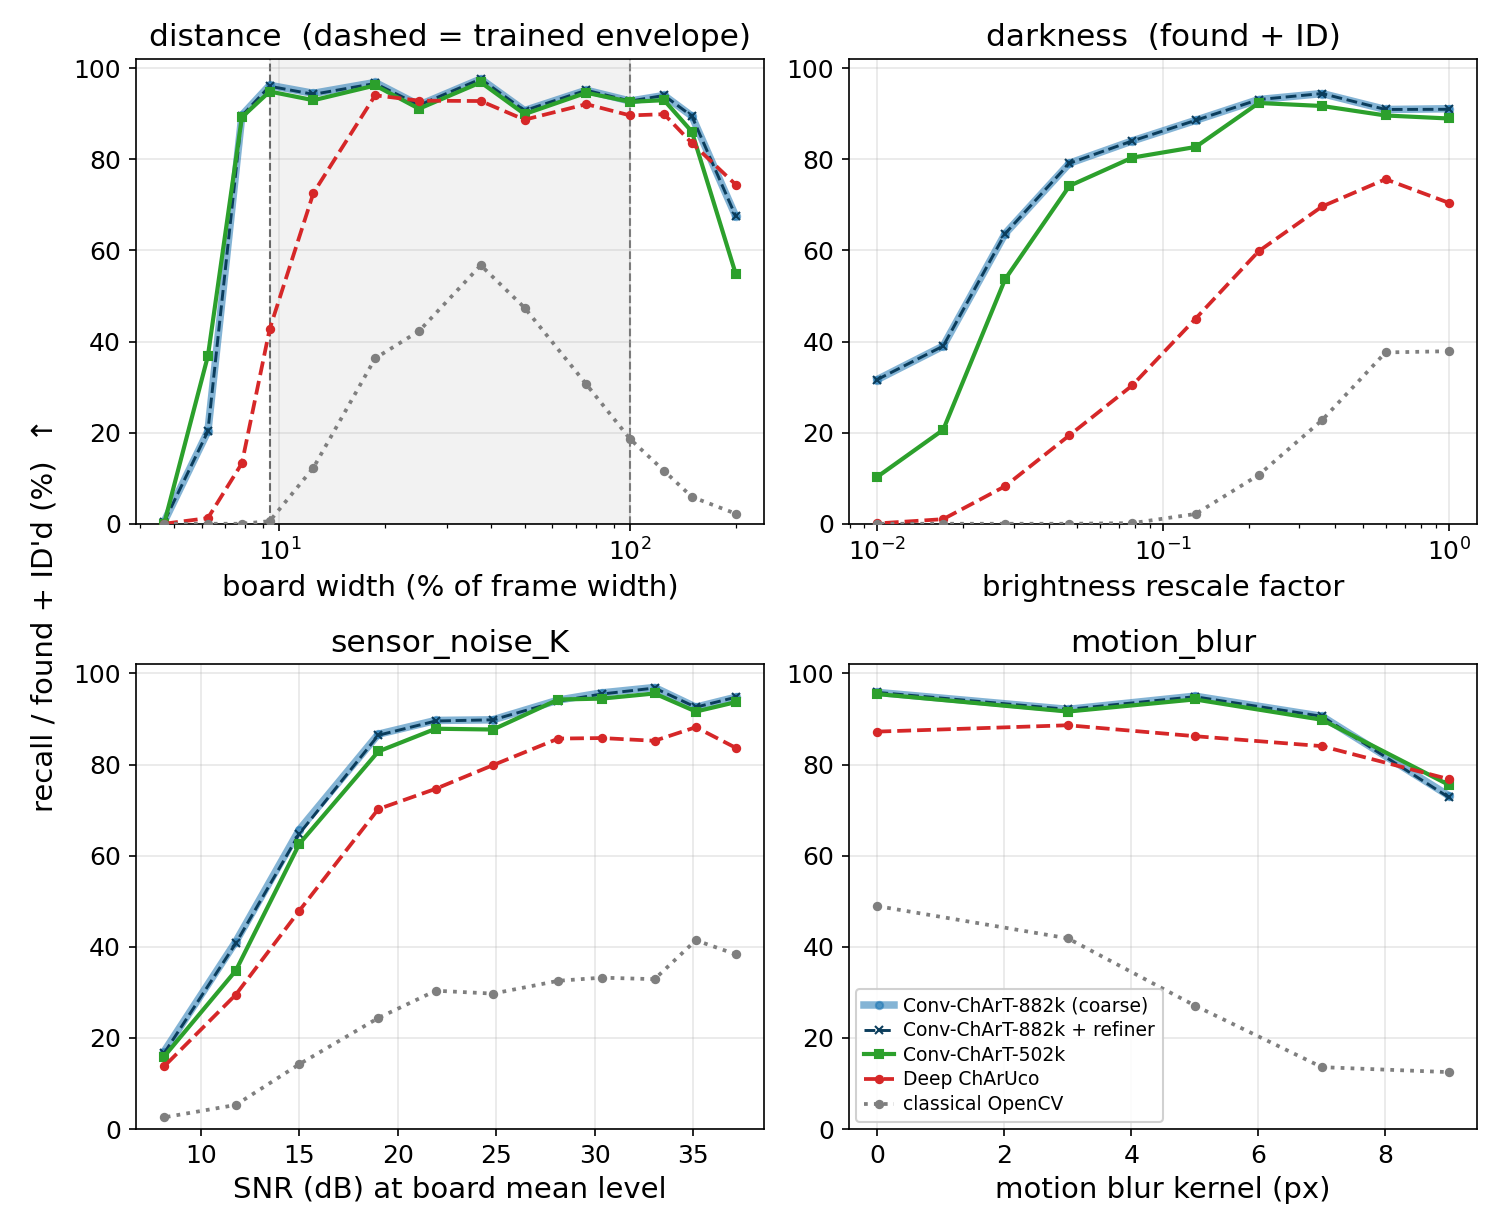
\includegraphics[width=0.98\textwidth]{figs/fourway_PANEL_recallrelease.png}
\caption{\textbf{Detection recall across four degradation axes}, on identical frames. The classical
pipeline degrades first on every axis; Conv-ChArT retains recall furthest into distance and low
light.}
\label{fig:panel}
\end{figure*}

\begin{table}[t]
\centering\small
\setlength{\tabcolsep}{3pt}
\begin{tabular}{lrrrrr}
\toprule
Factor & 222k & 502k & 882k & DC & Cls. \\
\midrule
Distance $s{=}128$ & 91.7 & 92.6 & 92.8 & 89.6 & 18.6 \\
Darkness & 5.6$^\dagger$ & 37.3 & 45.8 & 0.2 & 0.0 \\
Sensor noise & 16.5 & 15.4 & 16.6 & 13.8 & 2.6 \\
Motion blur & 63.6 & 75.3 & 72.8 & 76.8 & 12.5 \\
Ink contrast & 54.9 & 63.6 & 70.3 & 58.5 & 11.3 \\
Object occl. $\times4$ & 92.8 & 94.2 & 96.0 & 87.5 & 32.8 \\
Board occl. 50\% & 82.3 & 87.1 & 85.9 & 73.1 & 9.6 \\
Tilt 60\dgr & 91.5 & 91.9 & 92.7 & 90.0 & 51.6 \\
\bottomrule
\end{tabular}
\caption{Detection recall (\%) at the most severe step of each factor, for eight of the twenty
factors measured; the full set is listed in Appendix~\ref{app:abl}. Bold marks the best value in a
row; $\dagger$ marks a value discussed in the text for being anomalous rather than best.
DC = Deep ChArUco, Cls. = classical.}
\label{tab:robust}
\end{table}

Figure~\ref{fig:panel} and Table~\ref{tab:robust} report twenty degradation factors on identical
frames. The classical pipeline's identity column is ${\sim}100\%$ by construction, since it reports
only corners it has already decoded; its recall is the informative column.

\textbf{Capacity buys identity under degradation.} Board occlusion is the clearest case: identity
accuracy spans 40.2\%$\rightarrow$56.8\%$\rightarrow$71.2\% across our tiers, a 31\,pp separation on
frames where clean validation separates the same models by 0.44\,pp. Clean-set metrics
substantially understate what additional capacity provides.

\textbf{A deployment caution.} The smallest tier collapses to 5.6\% recall at the most severe
darkness step, against 37.3\% and 45.8\% for the larger tiers. This is a cliff rather than a
graceful decline, and it is invisible in clean-validation numbers.

\subsection{Efficiency and deployment}
\label{sec:deploy}

All four networks export to ONNX opset 17 with no operator outside the standard embedded-runtime
set (detectors 284/263/263 nodes at 2.05/3.70/5.74\,MB; refiner 20 nodes at 0.37\,MB) and agree
with the reference implementation to ${\sim}10^{-4}$ in logit space. Half-precision behaviour
separates by stage: applying fp16 to each network independently displaces 3 corners (0.062\%)
beyond 0.05\,px for the detector alone and 41 (0.846\%) for the refiner alone, additively
recovering the 44 (0.908\%) observed when both are quantised. The refiner accounts for the entire
sub-pixel displacement tail and none of the identity change. Retaining the 97,056-parameter refiner
at full precision while quantising the detector reduces the displaced fraction to 0.008--0.067\%;
uniform quantisation of both networks fails our acceptance criterion at every tier. That
criterion, fixed before the measurement, is that fewer than 0.1\% of corners may be displaced by
more than 0.05\,px and identity may change on fewer than 0.1\%. We note that
``fp32'' convolutions execute in TF32 by default on current hardware, whose 10-bit mantissa matches
fp16's; a comparison against an undisabled TF32 reference understates the effect.

\subsection{Ablation studies}
\label{sec:ablation}

Every arm differs from its control by exactly one configuration key, verified programmatically
before launch, and is trained to a matched budget on an identical data stream. Deltas are quoted
against the control of the same width and budget, and against that width's reproducibility floor.
Appendix~\ref{app:abl} reports the remaining studies.

\textbf{Reproducibility floor.}
\label{sec:abl_floor}
We train repeated seeds of an identical configuration and take the range of the final
10,000-sample validation (Table~\ref{tab:floor}). The floor is a joint property of width and
metric: the p95 range at 882k is $11.6\times$ tighter than at 222k, and the refiner resolves median
error $55\times$ more finely than its own p95. Two consequences follow. First, at 222k an identity
range of 6.18\,pp exceeds every effect we measure at that width, so we draw no conclusions there.
Second, mid-training ranges are far larger than final ones: on the in-loop 2000-sample validation
the 502k four-seed identity range is 35.39\,pp at step 7500, against 0.09\,pp on the full set at
step 35,000. Intermediate validations therefore measure which seed converged first, not which
configuration is better.

\begin{table}[t]
\centering\small
\begin{tabular}{lrrr}
\toprule
Width & Seeds & M-04 range & p95 range \\
\midrule
222,138 & 4 & 6.18\,pp & 0.0231\,px \\
502,322 & 4 & 0.09\,pp & 0.0061\,px \\
882,402 & 3 & 0.07\,pp & 0.0020\,px \\
Refiner (97,056) & 3 & med.\ 0.0017\,px & p95 0.0940\,px \\
\bottomrule
\end{tabular}
\caption{Seed-to-seed range of an identical configuration, on the full 10,000-sample validation
at the 35,000-step ablation budget. Applied to the released 100,000-step models of
Table~\ref{tab:detector} it is indicative rather than exact, since reproducibility is itself a
function of budget.}
\label{tab:floor}
\end{table}

\textbf{Attention bottleneck.}
\label{sec:abl_attn}
\emph{W/o attention} replaces the two transformer blocks with an equal-depth convolutional stack,
leaving encoder, decoder and heads unchanged. At 4.7M parameters and matched budget it gives
98.25\% identity against 98.80\% for the control, and the deficit concentrates at large $s$, where
a corner's own neighbourhood contains no marker and identity must come from board-scale context.
Within the bottleneck, halving the head count, halving the attention resolution (which \emph{adds}
607k parameters), removing one of the two blocks, and changing the rotary wavelength anchor all lie
within the 0.0020\,px / 0.07\,pp floor for this width (Table~\ref{tab:ab_arch}). The bottleneck is
therefore necessary but already at its smallest useful configuration, which is what permits the
parameter budget of Table~\ref{tab:params}.

\textbf{Supervision signal.}
\label{sec:abl_sup}
\emph{W/o one-hot supervision} restores the convention of~\cite{cornernet}: a Gaussian heatmap
target of width $\sigma_{\mathrm{hm}}$ under Eq.~\ref{eq:focal}. Sweeping $\sigma_{\mathrm{hm}}$ to
the one-hot limit at the reference width and matched budget gives 0.7781, 0.7352, 0.7335 and
\textbf{0.6970}\,px p95 at $\sigma_{\mathrm{hm}} = 1.0$, 0.5, 0.25 and one-hot respectively, with
identity varying by 0.14\,pp across the Gaussian rungs, twice this width's floor but an order of
magnitude below the localisation effect, and the tail improving $8.8\times$ at the limit. The
mechanism is that the graded target enters the loss only through the $(1-Y)^{\beta}$ factor on the
negative branch: at $\sigma_{\mathrm{hm}}=2$, $\beta=4$, a pixel one pixel from a corner has
$Y \approx 0.8825$ and therefore weight $1.9\times10^{-4}$, so displaced probability mass is nearly
free. Measured on identical frames ($n=830$), peaks under Gaussian supervision have RMS radius
1.0028\,px with 26.1\% of local mass on the peak pixel, against 0.2665\,px and 93.5\% under one-hot
supervision; since localisation decodes an argmax, a broader peak is directly a noisier estimate.
Setting $\beta=0$ isolates the two terms of Eq.~\ref{eq:focal}: it recovers 76.6\% of the
localisation gain but only 8.5\% of the identity gain, so the proximity discount governs
localisation and the easy-example modulation governs identity, which is why the two heads are
supervised differently. Full ladders are in Appendix~\ref{app:abl}.

\textbf{Geometric gating.}
\label{sec:abl_gate}
\emph{W/o the confidence gate} applies the refiner to every crop. This raises the 95th-percentile
refinement error from 0.761\,px to 3.011\,px while moving the median by 0.0012\,px: the refiner is
worse than the coarse peak on 16.3\% of crops, of which 55\% are featureless (intensity standard
deviation $<15$, against 20\% of the remainder), and the gate fires on 13.8\% of crops and is
correct 69.5\% of the time. \emph{W/o the lattice gate} passes all identified corners to PnP
without the consistency test, which is the configuration the learned baseline is effectively in;
Table~\ref{tab:pose} shows the consequence, a 95th-percentile rotation error of 89.36\dgr\ against
1.17\dgr. Neither gate improves the median: both truncate the tail, which is the property that
matters when poses are consumed without inspection.

%---------------------------------------------------------------
\section{Discussion}

\textbf{Limitations.} Training is entirely synthetic; we have not evaluated on annotated real
imagery, and the photometric model, while calibrated to a specific sensor class, is a model. The
pose evaluation sets omit the segmentation-derived object occluders used in training, so object
occlusion is characterised only on its own robustness axis. The classical baseline is evaluated at
default parameters, and a practitioner-tuned configuration would likely improve its recall.

\textbf{Uncertainty.} Our per-corner scale estimate is a useful ordering signal but is not a
variance, and the pose covariance is approximately $6\times$ over-confident. We report this rather
than applying a fitted inflation factor, which would conceal the mis-specification rather than
correct it.

\textbf{Scope of the null results.} The structural variants in Appendix~\ref{app:abl} are
established within our operating envelope, board geometry and data distribution, at the sample
sizes stated. They are not claims about attention in dense prediction generally.

%---------------------------------------------------------------
\section{Conclusion}

We presented Conv-ChArT, a convolutional--transformer hybrid for ChArUco corner detection and pose
estimation that establishes a new accuracy--efficiency operating point for this task. Our full
pipeline is $2.3\times$ smaller than the prior learned state of the art while reducing median
rotation error $6.9\times$, and a $7.0\times$ smaller variant still surpasses it on every accuracy
metric. Two design choices account for this. Abstention is geometric and explicit, bounding the
error distribution rather than merely lowering its centre; and the supervision departs from the
dense-keypoint convention in a way that measurably sharpens the decoded peak. Reporting every
ablation against a measured reproducibility floor is what allowed us to size the network by
evidence rather than convention, and we recommend the practice wherever reported effects are small
relative to training stochasticity.

%---------------------------------------------------------------
\begin{thebibliography}{99}\small
\bibitem{artoolkit} H.~Kato and M.~Billinghurst. Marker tracking and HMD calibration for a
video-based augmented reality conferencing system. \emph{IWAR}, 1999.
\bibitem{artag} M.~Fiala. ARTag, a fiducial marker system using digital techniques. \emph{CVPR},
2005.
\bibitem{apriltag} E.~Olson. AprilTag: A robust and flexible visual fiducial system. \emph{ICRA},
2011.
\bibitem{aruco} S.~Garrido-Jurado et al. Automatic generation and detection of highly reliable
fiducial markers under occlusion. \emph{Pattern Recognition}, 2014.
\bibitem{hu2019} D.~Hu, D.~DeTone, and T.~Malisiewicz. Deep ChArUco: Dark ChArUco marker pose
estimation. \emph{CVPR}, 2019.
\bibitem{cornernet} H.~Law and J.~Deng. CornerNet: Detecting objects as paired keypoints.
\emph{ECCV}, 2018.
\bibitem{centernet} X.~Zhou, D.~Wang, and P.~Kr\"ahenb\"uhl. Objects as points.
\emph{arXiv:1904.07850}, 2019.
\bibitem{unet} O.~Ronneberger, P.~Fischer, and T.~Brox. U-Net: Convolutional networks for
biomedical image segmentation. \emph{MICCAI}, 2015.
\bibitem{attnunet} O.~Oktay et al. Attention U-Net: Learning where to look for the pancreas.
\emph{MIDL}, 2018.
\bibitem{roformer} J.~Su et al. RoFormer: Enhanced transformer with rotary position embedding.
\emph{Neurocomputing}, 2024.
\bibitem{ropevit} B.~Heo et al. Rotary position embedding for vision transformers. \emph{ECCV},
2024.
\bibitem{ippe} T.~Collins and A.~Bartoli. Infinitesimal plane-based pose estimation. \emph{IJCV},
2014.
\bibitem{foi2008} A.~Foi et al. Practical Poissonian--Gaussian noise modeling and fitting for
single-image raw-data. \emph{IEEE TIP}, 2008.
\end{thebibliography}

\appendix
\onecolumn

%---------------------------------------------------------------
\section{Extended implementation details}
\label{app:impl}

\textbf{Architecture.} Encoder widths at multiplier 0.5 are 16/32/64/128 channels across stages
e1--e4, each a pair of $3\times3$ Conv--BN--ReLU with stride-2 downsampling between stages. The
bottleneck operates on the $H/8$ map at embedding dimension 256 with 8 heads, MLP ratio 4,
LayerNorm $\varepsilon = 10^{-6}$, no dropout, and qkv bias enabled. Rotary embedding uses 8
frequencies per axis over 16 dimensions per axis, with fp32 phase buffers. The decoder uses
bilinear upsampling followed by $3\times3$ convolution, with skip concatenation at each rung. The
refiner is $3\times3$ conv $1\rightarrow32$, $32\rightarrow64$, $64\rightarrow64$ at $24^2$, a
centre crop to $8\times8$, $3\times3$ $64\rightarrow64$, $1\times1$ $64\rightarrow64$ logits, then
PixelShuffle$(8)$ to $64\times64$.

\textbf{Training.} Batch 16 with accumulation 2; AdamW $\beta = (0.9, 0.999)$; peak learning rate
$3\times10^{-4}$, floor $3\times10^{-6}$, cosine schedule anchored to the total step budget, 1000
warmup steps; weight decay $10^{-4}$ applied to neither biases nor normalisation parameters;
gradient clipping at 5.0; EMA decay 0.999, evaluated in place of the live weights. Mixed precision
is bf16 with fp32 master weights. The data loader uses a spawn start method, 12 workers, prefetch
factor 4, and single-threaded OpenCV per worker. Validation runs every 2500 steps on a fixed
2000-sample subset and every 25,000 steps on the full 10,000-sample set; all reported numbers are
from the full set.

\textbf{Determinism and provenance.} Every sampler takes an explicit random generator; the codebase
contains no global random-number use, enforced by a static scan in the test suite. A content hash
of the generator sources and of the configuration subset that shapes their output is recorded with
every checkpoint, and training refuses to start if either has drifted since the last passing data
audit. Reported detection numbers are single runs; the seed spread of an identical configuration is
quantified in Table~\ref{tab:floor} and should be read as the uncertainty on any single number.

%---------------------------------------------------------------
\section{Synthetic data generation}
\label{app:data}

\textbf{Photometric model.} Applied in a pinned order, each stage independently gated by its own
probability: illumination, occlusion, specular lobe, refractive droplets, vignette, near-infrared
ink-contrast jitter, blur family (motion and defocus), Poissonian--Gaussian sensor
noise~\cite{foi2008}, fixed-pattern noise, speckle, and contrast. The model targets an industrial
global-shutter monochrome camera with a narrow-band near-infrared filter and no consumer
image-signal-processor stages.

\textbf{Reported signal-to-noise ratio is that of the delivered frame.} Noise is drawn per colour
channel before grayscale conversion, and the luminance-weighted average of three independent draws
attenuates the delivered standard deviation by
$\sqrt{0.114^2 + 0.587^2 + 0.299^2} = 0.6686$, measured 0.6676--0.6789 over
$\sigma \in [3,12]$\,DN. The delivered frame is therefore 3.50\,dB quieter than the per-channel
Poissonian--Gaussian formula implies, and we report the delivered figure.

\textbf{Labelling policy.} Corner visibility is geometric only: a corner is visible if it lies in
frame and outside every occluder. Photometric degradation never changes a label, which keeps the
label a function of geometry alone and prevents the network being supervised to hallucinate corners
it cannot see. A corner whose crop is illegible retains its true index, so the class loss on
illegible corners is reducible only through the attention pathway.

%---------------------------------------------------------------
\section{Further ablations}
\label{app:abl}

All arms are trained to a matched budget with exactly one configuration key changed, and are
compared against the control of the same width. Values are p95 (px), M-04 (\%) and tail (\%).

\textbf{The twenty degradation factors.} Each factor is swept over a ladder of severity steps on
frames that are otherwise bit-identical across methods and steps, so that only the swept parameter
varies. The factors are: \emph{geometric} --- distance ($s = 12$ to 128\,px), distance-extrapolated
($s = 6$ to 256, outside the trained envelope), rotation, tilt; \emph{photometric} --- brightness,
darkness, contrast, ink contrast, vignette, specular, droplets; \emph{sensor} --- sensor noise
(gain $K$), motion blur, defocus blur; \emph{occlusion} --- board occlusion (percentage of board
area), object occlusion (segmentation-derived cutouts), rectangular occlusion; and
\emph{differencing} --- differencing ratio, differencing ambient level, differencing ghosting.
Table~\ref{tab:robust} reports eight of these, chosen to span all five groups; the remaining twelve
follow the same qualitative pattern and are included in the released result set. The severity
ladders are defined in the released sweep configuration rather than reproduced here.

\textbf{Heatmap target and loss form.} Table~\ref{tab:ab_hm} gives the target-width ladder at the
reference width and the loss decomposition at 4.7M parameters.

\begin{table}[h]
\centering\small
\begin{minipage}{0.46\textwidth}\centering
\begin{tabular}{lrrr}
\multicolumn{4}{c}{(a) 882,402 params, 35k steps}\\
\toprule
Target & p95 & M-04 & Tail \\
\midrule
Gaussian $\sigma_{\mathrm{hm}}{=}1.0$ & 0.7781 & 98.90 & 0.1006 \\
Gaussian $\sigma_{\mathrm{hm}}{=}0.5$ & 0.7352 & 98.86 & 0.0849 \\
Gaussian $\sigma_{\mathrm{hm}}{=}0.25$ & 0.7335 & 99.00 & 0.0803 \\
One-hot & \textbf{0.6970} & \textbf{99.29} & \textbf{0.0114} \\
\bottomrule
\end{tabular}
\end{minipage}\hfill
\begin{minipage}{0.52\textwidth}\centering
\begin{tabular}{lrrr}
\multicolumn{4}{c}{(b) 4,698,034 params, 50k steps}\\
\toprule
Supervision & p95 & M-04 & Tail \\
\midrule
$\sigma_{\mathrm{hm}}{=}2.0$, focal $\beta{=}4$ & 0.8149 & 98.80 & 0.1221 \\
$\sigma_{\mathrm{hm}}{=}1.0$, focal $\beta{=}4$ & 0.7430 & 99.06 & 0.0687 \\
$\sigma_{\mathrm{hm}}{=}0.25$, focal $\beta{=}4$ & 0.7016 & 99.05 & 0.0392 \\
$\sigma_{\mathrm{hm}}{=}2.0$, $\beta{=}0$ & 0.7032 & 98.87 & 0.0463 \\
One-hot, BCE & \textbf{0.6690} & \textbf{99.62} & \textbf{0.0056} \\
\bottomrule
\end{tabular}
\end{minipage}
\caption{Heatmap target width and loss decomposition.}
\label{tab:ab_hm}
\end{table}

\textbf{Per-head supervision.} The two heads need not share a loss form
(Table~\ref{tab:ab_perhead}). At 882k, one-hot BCE on the heatmap improves p95 under either
class-head setting, and focal on the class head gives the best p95 and tail of the four. At 222k the
same combination collapses identity to 58.54\%, far outside that width's 6.18\,pp range, which is
why it is not carried to that tier.

\begin{table}[h]
\centering\small
\begin{tabular}{llrrr}
\toprule
Heatmap loss & Class loss & p95 & M-04 & Tail \\
\midrule
\multicolumn{5}{l}{\emph{882,402 params, 35k steps}}\\
focal (Gaussian) & focal (Gaussian) & 0.7352 & 98.86 & 0.0849 \\
focal (Gaussian) & BCE (one-hot) & 0.7572 & 99.00 & 0.0931 \\
BCE (one-hot) & focal (Gaussian) & \textbf{0.6874} & 98.87 & \textbf{0.0081} \\
BCE (one-hot) & BCE (one-hot) & 0.6970 & \textbf{99.29} & 0.0114 \\
\midrule
\multicolumn{5}{l}{\emph{222,138 params, 35k steps}}\\
focal (Gaussian) & focal (Gaussian) & 0.8096 & 94.87 & 0.0952 \\
focal (Gaussian) & BCE (one-hot) & 0.8222 & 96.71 & 0.1265 \\
BCE (one-hot) & focal (Gaussian) & 0.7430 & 58.54$^\dagger$ & 0.0182 \\
BCE (one-hot) & BCE (one-hot) & 0.7611 & 94.76 & 0.0218 \\
\bottomrule
\end{tabular}
\caption{Per-head loss form, crossed at two widths, 35k steps. Bold marks the best value in a
column within each width block; $\dagger$ marks the identity collapse discussed in the text.}
\label{tab:ab_perhead}
\end{table}

\textbf{Head balance.} $\lambda_{\mathrm{cls}}$ scales the class-head term of Eq.~\ref{eq:total}.
At 882k it is a trade at every setting, buying identity at roughly 0.06\,px of p95 per point; at
502k it is free within the measured range, which is why the released tiers differ
(Table~\ref{tab:ab_lambda}).

\begin{table}[h]
\centering\small
\begin{tabular}{lrrrr}
\toprule
Width & $\lambda_{\mathrm{cls}}$ & p95 & M-04 & Tail \\
\midrule
882,402 & 1.5 & 0.7021 & 99.34 & 0.0130 \\
882,402 & 2.0 & 0.7059 & 99.40 & 0.0098 \\
882,402 & 4.0 & 0.7143 & 99.51 & 0.0115 \\
\midrule
502,322 & 1.5 & 0.7122 & 98.98 & 0.0124 \\
502,322 & 2.0 & 0.7208 & 99.09 & 0.0140 \\
502,322 & 3.0 & 0.7234 & 99.12 & 0.0165 \\
502,322 & 4.0 & 0.7262 & 99.29 & 0.0124 \\
\midrule
222,138 & 0.5 & 0.7318 & 91.96 & 0.0192 \\
222,138 & 2.0 & 0.7580 & 97.80 & 0.0168 \\
222,138 & 4.0 & 0.7703 & 97.78 & 0.0168 \\
\bottomrule
\end{tabular}
\caption{Class-head weight, 35k steps.}
\label{tab:ab_lambda}
\end{table}

\textbf{Class-target and refiner-target width.} In contrast to $\sigma_{\mathrm{hm}}$, the
class-target width is null in both directions: at 502k, $\sigma_{\mathrm{cls}}=0.5$ gives
0.7110 / 98.87 and $\sigma_{\mathrm{cls}}=2.0$ gives 0.7104 / 98.80, both within that width's range
of the 0.7139 / 98.80 control. The class map is at $H/4$, so one cell spans four input pixels and
sub-pixel structure in its target is not recoverable. The refiner-target width is likewise null
(median 0.0937 against 0.0969\,px at $\sigma_{\mathrm{ref}} = 0.75$ and 1.5), against a median
range of 0.0017\,px but a p95 range of 0.0940\,px that cannot arbitrate the p95 column.

\textbf{Attention bottleneck internals.} Table~\ref{tab:ab_arch} varies the bottleneck against a
matched control at the reference width. All four variants lie within the 0.0020\,px / 0.07\,pp
floor, so we retain the smallest configuration.

\begin{table}[h]
\centering\small
\begin{tabular}{lrrr}
\toprule
Variant (882,402 params, 35k steps) & p95 & M-04 & Tail \\
\midrule
Control (8 heads, $H/8$, 2 blocks) & 0.7352 & 98.86 & 0.0849 \\
4 heads & 0.7359 & 98.77 & 0.0746 \\
Attention at $H/16$ ($+607$k params) & 0.7398 & 98.96 & 0.0586 \\
1 block & 0.7398 & 98.51 & 0.0803 \\
RoPE anchor $\lambda_{\min}{=}5$ cells & 0.7400 & 98.89 & 0.0794 \\
\bottomrule
\end{tabular}
\caption{Attention bottleneck variants.}
\label{tab:ab_arch}
\end{table}

\textbf{Skip gating.} \emph{W/o gate} removes the additive attention gate on the $H/4$ skip,
passing the encoder features through unmodified. This changes p95 by $-0.0011$ at 882k
(0.6959 against 0.6970) and $+0.0018$ at 502k, both within range. Adding a second gate on the $H/8$
skip gives 0.7063 / 98.89 at 502k against 0.7139 / 98.80 for the control, i.e.\ $1.2\times$ and
$1.0\times$ the respective ranges. Gating is retained on the $H/4$ skip only, at 6209 parameters.

\textbf{Encoder dilation, cross-scale attention and width.} At 4.7M parameters and 50k steps,
removing the dilated cascade from the deepest encoder stage gives 0.8072 / 98.77 against the
0.8149 / 98.80 control while removing 25\% of parameters; adding cross-scale attention gives
0.8148 / 98.82; disabling gates gives 0.8134 / 98.88. Halving the width gives 0.8605 / 98.67, the
only structural change with an effect clearly outside the range, and it is a degradation.

\textbf{Optimisation.} Raising the peak learning rate from $3\times10^{-4}$ to $6\times10^{-4}$
gives 0.7100 / 99.30 against 0.7238 / 98.10 at $1.5\times10^{-4}$, at 502k and 35k steps. We retain
$3\times10^{-4}$ for the released models, whose longer schedule alters the comparison.

\textbf{Composite configurations.} Levers do not compose additively. Combining the two-gate
topology with $\lambda_{\mathrm{cls}}=2$ at 222k gives 0.7624 / 97.25, worse on both axes than
$\lambda_{\mathrm{cls}}=2$ alone (0.7580 / 97.80). At 882k, one-hot heatmap with focal class head
and $\lambda_{\mathrm{cls}}=2$ gives 0.6894 / 99.15 with a tail of 0.0065\%, the best tail measured
at that width and the configuration we release.

\textbf{Training budget.} Our 502,322-parameter model at 100,000 steps (0.6885 / 99.41) outperforms
the 882,402-parameter model at the 35,000-step ablation budget (0.6894 / 99.15) on both axes.
Ablation deltas are valid at matched budget; absolute ablation values are budget-limited and should
not be compared with the released models of Table~\ref{tab:detector}.

\end{document}
